%       10        20        30        40        50        60       70        80        90        100
%234567890123456789012345678901234567890123456789012345678901234567890123456789012345678901234567890

\documentclass[dvipsnames,12pt]{article} % \documentclass{article}
\usepackage[utf8]{inputenc}
\usepackage{graphicx} % Required for inserting images
\usepackage{enumitem}
\usepackage{float}
%%%%%%%%%%%%%%%%%%%%%%%%%%%%%%%%%%%%%%%%%%%%%%%%%%%%%%%%%%%%%%%%%%%%%%%%%%%%%%%%%%%%%%%%%%%%%%%%%%%%
%%%%%%%%%%%%%%%%%%%%%%%%%%%%%%  2024 WQ MATH 167 FPP REPORT TEMPLATE %%%%%%%%%%%%%%%%%%%%%%%%%%%%%%%
%%%%%%%%%%%%%%%%%%%%%%%%%%%%%%%%%%%%%%%%%%%%%%%%%%%%%%%%%%%%%%%%%%%%%%%%%%%%%%%%%%%%%%%%%%%%%%%%%%%%

% UNTIL SQ 2016 THIS WAS PROBLEM ?? IN HW 08

% MATH 167
% FALL QUARTER 2024
% 184 YOUNG HALL
%
%   Tue Mar 12 11:30:36 AM PDT 2024
%
%     REVISION HISTORY:
%
%       REVISION 1.00
%
%         Revision 1.00: Tue Mar 12 11:30:36 AM PDT 2024
%         Revision 1.01: Tue Mar 12 07:52:05 PM PDT 2024
%         Revision 1.02: Wed Mar 13 06:57:30 PM PDT 2024
%         Revision 1.03: Fri Mar 15 04:26:00 PM PDT 2024
%         Revision 1.04:
%         Revision 1.05:

%%%%%%%%%%%%%%%%%%%%%%%%%%%%%%%%%%%%%% SET UP PAGE PARAMETERS %%%%%%%%%%%%%%%%%%%%%%%%%%%%%%%%%%%%%%

% EGP's preferred page style for notes, homework assignments, exams, etc.

% Margins, paragraph indents, space between paragraphs if any, etc. Good references
% include page 85 of "The LaTeX Companion" by Frank Mittelbach and Michel Goossens and
% page 260 of "Math Into LaTeX" by George Gratzer.

% Enlarge the width and height of the printed page

\setlength{\textwidth }{08.00 in} % EGP's default is \textwidth   = 6.50 in
\setlength{\textheight}{09.25 in} % EGP's default is \textheight  = 9.25 in

% Space between the end of the odd and even side margins and the beginning of the text.

\setlength{\oddsidemargin }{0.0 in}
\setlength{\evensidemargin}{0.0 in}

% The side margins are 1.0 inch plus \hoffset and the top margins is 1.0 inch plus
% \voffset. According to "The LaTeX Companion" the default values are \hoffset = 00 pt
% and \voffset = 00 pt.

\setlength{\hoffset}{-0.75 in} % EGP's default is \hoffset    = 00.00 in
\setlength{\voffset}{-0.50 in} % EGP's default is \voffset}   = -0.50 in

% If there is no header in this document, set each of the following values to zero.

% This is the amount of space between the BOTTOM of the HEAD and the TOP of the BODY.
% According to "Math Into LaTeX"  by George Gratzer the default values for LaTeX's
% article document is \headsep = 25 pt.

\setlength{\headsep}{12 pt}

% Package Fancyhdr Warning: \headheight = 12 pt is too small. Make it at least 14.0pt.
% According to "Math Into LaTeX"  by George Gratzer the default value for LaTeX's article
% document is \headheight = 12 pt.

\setlength{\headheight}{14 pt}

% This is the amount of space between the top of the page and the TOP of the header. According to "Math
% Into LaTeX"  by George Gratzer the default value for LaTeX's article document is \topmargin = 16 pt.
% \headheight = 12pt, and .

\setlength{\topmargin }{00 pt}

% This is the amount of space between the TOP OF THE BODY and THE BOTTOM OF THE FIRST
% line of text on the page. According to "Math Into LaTeX" by George Gratzer the default
% value for LaTeX's article documents is \topskip = ?? pt.

\setlength{\topskip}{12 pt}

% This is the amount of space between the last line on the page and the BOTTOM of the footer.
% According to https://en.wikibooks.org/wiki/LaTeX/Page_Layout the default value is
% \footskip = 30 pt.

\setlength{\footskip}{30 pt}

% I like space between paragraphs, since it makes the document more readable. However,
% this does not seem to change the spacing between paragraphs contained in an item of a
% list.

\setlength{\parskip}{12 pt} % default: \parskip        = 12  pt

% Comment out the following line to use the default amount to indent the first line of
% each paragraph.

\setlength{\parindent}{00 pt}

%%%%%%%%%%%%%%%%%%%%%%%%%%%%%%%%%%%%%% LOAD AMS LaTeX Packages %%%%%%%%%%%%%%%%%%%%%%%%%%%%%%%%%%%%%

\usepackage{amsmath}
\usepackage{amssymb}
\usepackage{amsfonts}

%%%%%%%%%%%%%%%%%%%%%%%%%%%%%%%%%%%% LOAD THE "enumitem" PACKAGE %%%%%%%%%%%%%%%%%%%%%%%%%%%%%%%%%%%

\usepackage{enumitem}

 \setenumerate[1]{labelindent=0pt,itemindent=00pt}

\setlength{\labelwidth}{00 pt}
\setlength{\leftmargin}{0.0in}

% As per the LaTeX Wiki book dvips knows a wider range of colors than xcolor alone (try 'svgnames')

\usepackage[dvipsnames]{xcolor}

% package to allow colored source code listings

\usepackage{listings}

% Format MATLAB code with the listings package

\usepackage{mcode}

% Create a language setting for LaTeX
% One can change the language for each code-block optionally
% \lstset
% {
%     language=[LaTeX]TeX,
%     breaklines=true,
%     basicstyle=\tt\scriptsize,
%     keywordstyle=\color{blue},
%     identifierstyle=\color{magenta},
% }


% I like space between paragraphs, since it makes the document more readable. However, this does not
% seem to change the spacing between paragraphs contained in an item of a list.

\setlength{\parskip}{03pt} % default: \parskip = 12  pt

\usepackage{color}   % May be necessary if you want to color links

%%%%%%%%%%%%%%%%%%%%%%%%%%%%%%%%%%%%% EGP's LOCAL LaTeX MACROS %%%%%%%%%%%%%%%%%%%%%%%%%%%%%%%%%%%%%

\newcommand{\bs}[1]{\boldsymbol{#1}}

%%%%%%%%%%%%%%%%%%%%%%%%%%%%%%%%%%%%%%%% EGP's COLOR MACROS %%%%%%%%%%%%%%%%%%%%%%%%%%%%%%%%%%%%%%%%

% dvips knows a wider range of colors than just xcolor

\usepackage[dvipsnames]{xcolor}

%%%%%%%%%%%%%%%%%%%%%%%%%%%%%%%%%%%%%%%% EGP's COLOR MACROS %%%%%%%%%%%%%%%%%%%%%%%%%%%%%%%%%%%%%%%%

% dvips knows a wider range of colors than just xcolor

\usepackage[dvipsnames]{xcolor}

\newcommand{\bl}[1]{{\textcolor{blue}{#1}}}
\newcommand{\Ma}[1]{{\textcolor{maroon}{#1}}}
\newcommand{\maroon}[1]{{\textcolor{Maroon}{#1}}}
\newcommand{\Nb}[1]{{\textcolor{NavyBlue}{#1}}}
\newcommand{\Og}[1]{{\textcolor{OliveGreen}{#1}}}
\newcommand{\rd}[1]{{\textcolor{red}{#1}}}
\newcommand{\Rm}[1]{{\textcolor[rgb]{0.69,0.19,0.38}{#1}}}
\newcommand{\Wr}[1]{{\textcolor{winered}{#1}}}

\newcommand{\Bb}[1]{{\textbf{\textcolor{Blue}{#1}}}} % Bold Face Blue
\newcommand{\Bg}[1]{{\textbf{\textcolor{Green}{#1}}}} % Bold Face Green
\newcommand{\BNb}[1]{\textbf{\Nb{#1}}} % Bold Face Navy Blue
\newcommand{\Bog}[1]{\textbf{\textcolor{OliveGreen}{#1}}}          % Bold Face Olive Green
\newcommand{\Brd}[1]{{\textbf{\textcolor{Red}{#1}}}}               % Bold Face Red
\newcommand{\Brp}[1]{\textbf{\textcolor{RoyalPurple}{#1}}}         % Bold Face Royal Purple
\newcommand{\Brm}[1]{\textbf{\textcolor[rgb]{0.69,0.19,0.38}{#1}}} % Bold Face Rich Maroon

\newcommand{\MATLAB}{\Bog{\textsc{MATLAB~}}}
\newcommand{\Python}{\Brm{Python~}}

% \renewcommand{\thefootnote}{\fnsymbol{footnote}} % A sequence of nine symbols, try it and see!

%%%%%%%%%%%%%%%%%%%%%%%%%%%%%%%% LOAD THE HYPERREF PACKAGE %%%%%%%%%%%%%%%%%%%%%%%%%%%%%%%

% The basic usage with the standard settings is straightforward. Just load the package in
% the preamble, at the end of all the other packages but prior to other settings.

% From the `Introduction' to the hyperref manual: Make sure it comes last of your loaded
% packages, to give it a fighting chance of not being over-written, since its job is to
% redefine many LATEX commands. Hopefully you will find that all cross-references work
% correctly as hypertext. For example, \section commands will produce a bookmark and a
% link, whereas \section* commands will only show links when paired with a corresponding
% \addcontentsline command.

% I think the default values for "bookmarks" is 'false' and for "bookmarksopen" is 'false'

\usepackage[bookmarksopen=false]{hyperref}

\hypersetup{colorlinks=true}

\hypersetup{linkcolor=blue}

\hypersetup{urlcolor=blue}

\hypersetup{linktoc=all}             % set to all if you want both sections and subsections linked

\hypersetup{pdftitle={2024 WQ CRN 30769 FPP REPORT TEMPLATE}}

\hypersetup{pdfcreator={\textcopyright 2024 The Authors}}

\hypersetup{pdfauthor={\textcopyright 2024 The Authors}}

%%%%%%%%%%%%%%%%%%%%%%%%%%%%%%%%%%%%%% TITLE, AUTHOR AND DATE %%%%%%%%%%%%%%%%%%%%%%%%%%%%%%%%%%%%%%

\title{2024 WQ Final Programming Project Report\footnote{Revision 1.03}}
\author{Your Name} %YOUR NAME
\date{\today}

\date{Fri Mar 15 04:26:00 PM PDT 2024}

\begin{document}

\maketitle
\tableofcontents
\newpage

  \section{PROBLEM DESCRIPTION}
    \label{SECT 01:PROBLEM DESCRIPTION}
    
      \Brd{(20 points total)}

      \vspace{06pt}

      I want you to provide \textbf{\textit{thoughtful}} responses to the prompts in this template.

      \vspace{06pt}

      As usual, in this section write a description of what you are doing and why it is useful or
      important.

      \vspace{06pt}

      You will find some helpful information in Chapter 10.01 of the first edition of the textbook.

      \vspace{06pt}

      There is also valuable information concerning this project, including background and history,
      here:
      \vspace{-02pt}
      \begin{center}
        \href{https://canvas.ucdavis.edu/files/23522088/download?download_frd=1}{NS\_LECTURE\_21}
      \end{center}
      \Brd{Do not plagiarize these lecture notes!} You may use the information in these lecture
      notes but \Brp{you must write this report entirely in your own words.}

      \vspace{06pt}

      Furthermore, your computer program must produce the required output for this report -
      including figures and confusion matrices - when the TA runs it.
      \Brd{(50 points - A separate from this section)}.

      \vspace{06pt}

      Even though the title of this section is ``Problem Description'' this is also where you
      \Brd{write the required} Introduction and Motivation.

      \vspace{06pt}

      \Brp{As always, keep in mind your intended audience .}
      Your report should be sufficiently detailed (and clear!) to give someone with an expert's
      understanding of (Numerical) Linear Algebra and computing, (but not necessarily the SVD)
      enough of an idea of what you did that they could reproduce your results.

      \vspace{06pt}

      \Brm{Make sure you address all of the following points.}

      \begin{enumerate}[label=\textbf{(\alph*}), leftmargin=48pt]

        \item \Brd{(05 points)} Introduction to and overview of the problem.

        \item \Brd{(05 points)} What are the objectives of this exercise or procedure on which you
          are reporting?

        \item \Brd{(05 points)} Why is it important?

        \item \Brd{(05 points)} Briefly mention where your report leads or ends up; i.e., briefly
          mention one or more conclusions.

        \item Keep this part concise and to the point.\\
        
       \vspace{06pt}
This project involves identifying the images of the handwritten digits data from a set of images. It is part of the computer vision. It is applied in a lot of scenarios in the real life, for example, character identification. This is important because in real life, we have a lot of images containing digits and we need to use computer to identify them.  In this project, we wil use Centriod Classification algorithm SVD method to identify the matrix images of digits, classify handwritten digits by rank-17 approximations. More importantly, we will compare the performance of two algorithms using matlab.
      \end{enumerate}

%Read the Introduction and Motivation section of the Sample Programming Project Report given to you for ideas.


  \section{DATA SET}
    \label{SECT 02:DATA}

      \Brd{(25 points total)}

      \vspace{06pt}

      Report on \textbf{Steps 01(a)-(b)} of the assignment.
        
%      \vspace{06pt}

      \begin{enumerate}[label=\textbf{(\alph*}), leftmargin=48pt]

%     \pdfbookmark[2]{Step~05~(a)}{Step_05_(a)}

        \vspace{06pt}

        \item \textbf{Step 01(a)}  \Brd{(05 points)} Briefly describe the data structure in which
          the images of the digits are stored.\\
          
        The dataset we are using is USPS.mat. We will extract the images of the digits and store them in train\_patterns and test\_patterns. Those variables are the matrix of 256* 4649 matrix, which means that for each digits images, it is 16*16= 256 pixels and there are 4649 images to be trained. We also have the corresponding train\_labels and test\_labels, which are matrix variables with normalized vectors, which means each number is from -1 to 1.
          
        
        \vspace{06pt}

        \item \textbf{Step 01(a)} \Brd{(05 points)} Include a (brief) explanation of the difference
          between the training data and the test data.
          (This is a simple example of \textit{machine learning}.)\\
        For training data, it is used for the computer to study and approach the result for machine learning. For test data, it is used to evaluate the overall result of learning. 
        \vspace{06pt}

        \item \Brd{(05 points)} Where can the data be obtained by a member of the general public;
          i.e., someone who \Brm{does not have access} to UCD CANVAS where you got your data.\\
          
          The handwritten digit data (similar to the one used here) can typically be found in public datasets like the MNIST database, link:http://www.gaussianprocess.org/gpml/data/ .

      \vspace{06pt}

      \item \textbf{Step 01(b)} \Brd{(05 points)} Display the first 16 images in train patterns.
        (Include this figure here.)
        \begin{figure}[H]
          \centering
          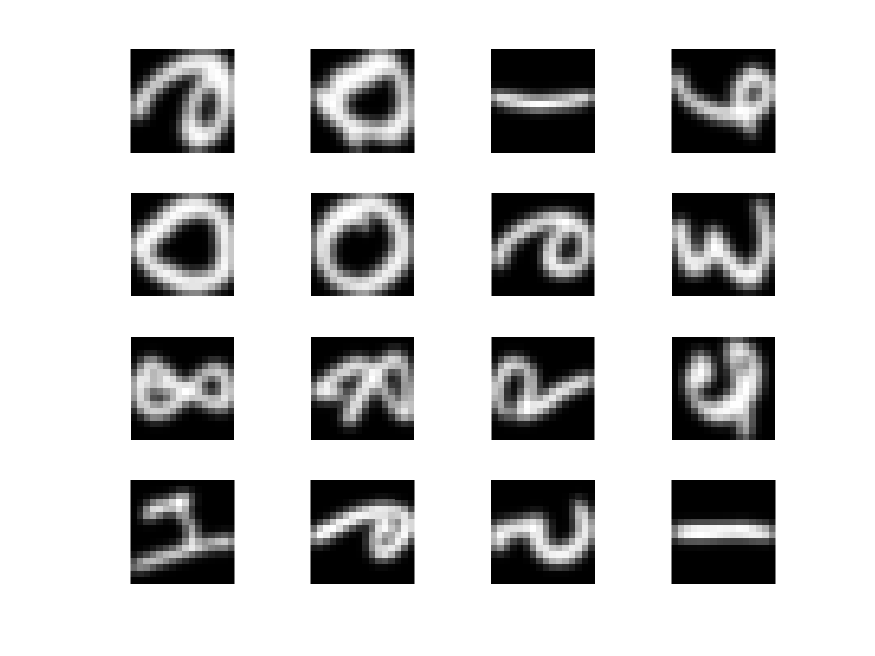
\includegraphics[width=0.8\textwidth]{digit_images.png}
          \label{fig:music}
        \end{figure}
      \vspace{06pt}

      \item \Brd{(05 points)} Write something brief but sensible about this figure; e.g., ``In
        Figure~01 we display ...''
        \Brd{\underline{Do not}} just plop the figure down on the page without writing something
         about it!\\
 From the figure, we can observe that the digits are: \\
        9 0 1 6\\
        0 0 9 3\\
        8 8 9 6\\
        4 6 5 1\\
    \end{enumerate}

  \section{THE CENTROID CLASSIFICATION ALGORITHM}
    \label{SECT 03:THE CENTROID ALGORITHM}

      \Brd{(05 points)}

      \vspace{06pt}

      \Brd{Include SEVERAL sentences here to introduce the Centroid algorithm.}
      For example, is this the most complicated algorithm that you can think of?
    The Centroid algorithm is used some center point to classify a set of data. It is an unsupervised learning algorithm for image recognition. 
      \subsection{DESCRIPTION OF THE ALGORITHM}
        \label{SUBSECT 3.1:CENTROID DESCRIPTION}
        
        \Brd{(15 points total)}
%       \textcolor{red}{(10 points)}

        \Brm{Report on Step 02 here.}

          \vspace{06pt}

        This section should be self explanatory.
        However, here are some prompts in case you want them.

%        \vspace{06pt}

%        \textcolor{red}{(05 points for each step)}
%         Report on Step 02

%        \vspace{06pt}

        \begin{enumerate}

          \item \Brd{(05 points)} Describe the algorithm in sufficient detail that your clone could
            reproduce your results based only on your description.\\
            1, initializing centroids by selecting random data points from the dataset.
            2, find the mean data for each image: the centroids of the clusters corresponding to each digit from 0 to 9.
          \item \Brd{(05 points)} Display the 10 mean digit images; i.e., place the figure here.
        \begin{figure}[H]
          \centering
          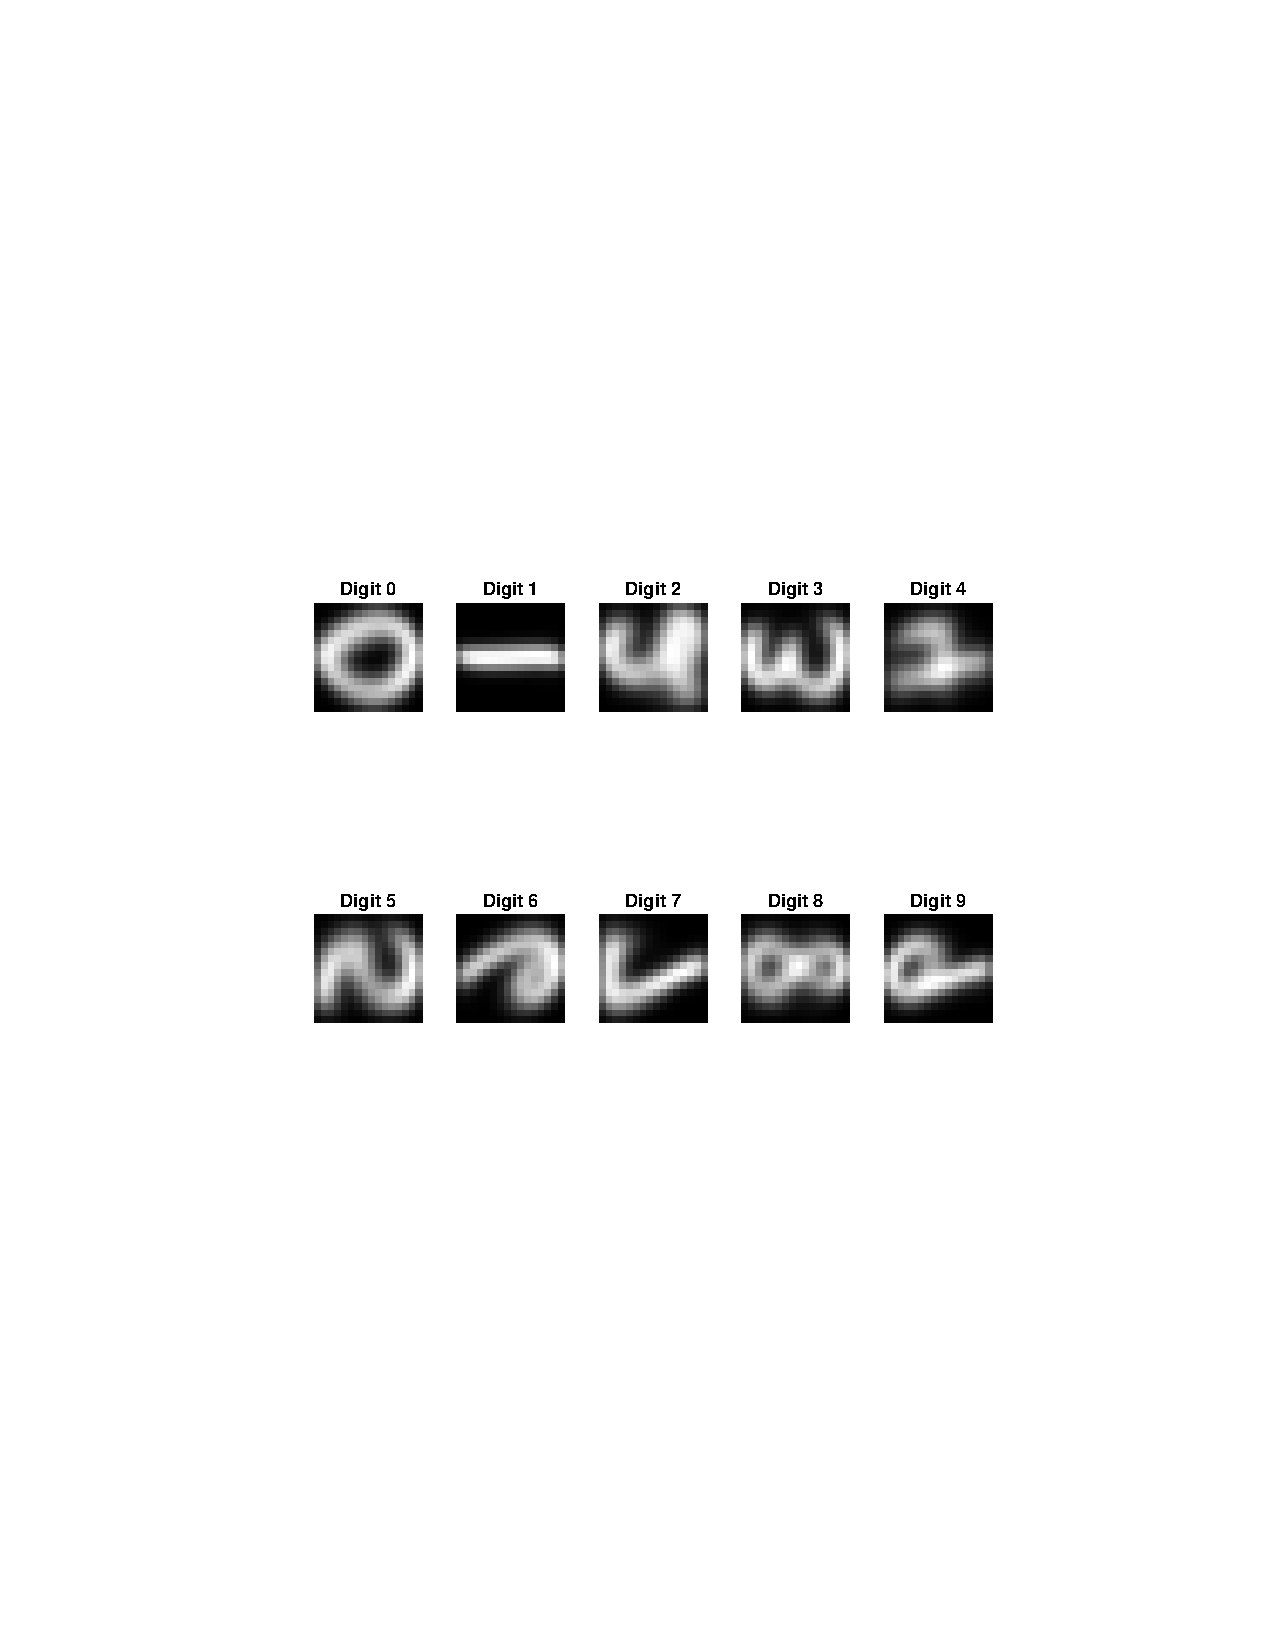
\includegraphics[width=0.8\textwidth]{mean_digits.pdf}
          \label{fig:music}
        \end{figure}
          \vspace{06pt}

          \item \Brd{(05 points)} Write something brief but sensible about the figure; e.g., ``In
          Figure~02 we display ...''
        From the figure, we observe that the images are from 0 to 9 respectively, which reaches the conclusion. 
        \end{enumerate}

      \subsection{DESCRIPTION OF THE RESULTS}
       \label{SUBSECT 3.2:CENTROID RESULTS}

        \Brm{Report on Step 03(b)--(c) here.}

          \vspace{06pt}

          \textcolor{red}{(05 points)}  Print the confusion matrix here.
          \Brd{Do not just leave the confusion matrix in this subsection without any text!}\\
          
          Here is confusion matrix of step 3:\\
        \begin{verbatim}    
    656     1     3     4    10    19    73     2    17     1
     0   644     0     1     0     0     1     0     1     0
    14     4   362    13    25     5     4     9    18     0
     1     3     4   368     1    17     0     3    14     7
     3    16     6     0   363     1     8     1     5    40
    13     3     3    20    14   271     9     0    16     6
    23    11    13     0     9     3   354     0     1     0
     0     5     1     0     7     1     0   351     3    34
     9    19     5    12     6     6     0     1   253    20
     1    15     0     1    39     2     0    24     3   314
        \end{verbatim}
          \vspace{06pt}

          \textcolor{red}{(05 points)}  Describe the confusion matrix.  For example,

          \begin{enumerate}

            \item  What is a confusion matrix?\\
            A confusion matrix is a result matrix describing the performance of a classification model on a set of test data for known values.

            \item What do the rows, columns, diagonal entries, represent?\\
            rows:the actual classes\\
            columns:the predicted classes\\
            Diagonal entries: the correctly classified instances for each class.\\
          \end{enumerate}

      \section{THE SVD CLASSIFICATION ALGORITHM}
        \label{SECT 04:SVD CLASSIFICATION ALGORITHM}
    
        \Brd{(05 points)}

        \vspace{06pt}

        \Brd{This is the beginning of Section 04! DO NOT LEAVE IT BLANK!}
        
        \vspace{06pt}

        Include several introductory sentences here.

        \vspace{06pt}

        Remember, the reader may not know what the SVD is.
        So you could start with something like the following.

        \vspace{06pt}

        The Singular Value Decomposition (SVD) is a powerful matrix factorization ...

        \subsection{DESCRIPTION OF THE ALGORITHM}
          \label{SECT 04.01:SVD DESCRIPTION}

          Report on \textbf{Steps 04(a)--(b)} in this Section.

          \vspace{06pt}

          \BNb{IMPORTANT!} This is the most technical section of your report.
          Try to \rd{{{clearly}}} explain the algorithm.
          (Don't hesitate to use equations.\footnote{An equation often communicates an idea better than a pile of words.})
          Your explanation should be sufficient to give someone with an expert's understanding of
          Numerical Linear Algebra - but not the SVD - a *basic* idea of what the SVD is and how
          the algorithm works.

%     \vspace{06pt}

          \begin{enumerate}[label=\textbf{(\alph*}), leftmargin=48pt]

%         \pdfbookmark[2]{Step~05~(c)}{Step_05_(c)}

            \item \textbf{Step 04(a)} \Brd{(10 points)} In your words and - if you like - equations
              describe Step 4(a).\\
            In Step 04(a), we compute the rank 17 SVD for each digit, which extracts all the digit images and compute the SVD matrix for all of them. The svd formula is $X_k=U_k\sum_kV_K^T$.
            
%          \pdfbookmark[2]{Step~05~(d)}{Step_05_(d)}

            \vspace{06pt}

            \item \textbf{Step 04(b)} \Brd{(10 points)} Similarly, in words and (possiby) equations
              describe Step 4(b).\\
            In Step 04(b), we compute the expansion coefficients of each digit image of test dataset with the 17 singular vectors of each train digit image set,respectively. We use the formula $c_{jk}=U_k^T*x_j$.
         \end{enumerate}

        \subsection{DESCRIPTION OF THE RESULTS}
          \label{SECT 04.02:SVD RESULTS}

          \begin{enumerate}[label=\textbf{(\alph*}), leftmargin=48pt]

   %         \pdfbookmark[2]{Step~05~(c)}{Step_05_(c)}

            \item \textbf{Step 04(c)} \Brd{(10 points)} In words
               and equations(?) describe Step 4(c).
               \begin{itemize}
               \item How do you compute the error and what is the rationale for doing it that way?
               \end{itemize}
                We compute the error between each original test dataset for digit image and its rank 17 approximation using the left singular vectors of the corresponding matrix.

   %          \pdfbookmark[2]{Step~05~(d)}{Step_05_(d)}

             \vspace{06pt}

             \item \textbf{Step 04(d)} \Brd{(10 points)} Print the confusion matrix.
               Describe this confusion matrix and what it tells you about the SVD algorithm's performance on this problem.

               \begin{itemize}
                 \item \Brd{(05 points)} For the correct confusion matrix and \Brd{(05 points)} for
                   your thoughts concerning what it tells you.
               \end{itemize}
               The confusion matrix will tell how well the SVD perform for the digit recognition, telling the number of test cases that were classified correctly and incorrectly

          \end{enumerate}

      \section{ANALYSIS}
        \label{SECT 05:ANALYSIS}

        \Brd{(20 points)}

        \vspace{06pt}

        \Bog{{STEP 05}} \textbf{Analyze your results!}

        \vspace{06pt}

        \Brm{Compare and contrast the Centroid and SVD Algorithms}

%       \vspace{06pt}

        \begin{enumerate}[label=\textbf{(\alph*}), leftmargin=48pt]

  %          \pdfbookmark[2]{Step~05~(c)}{Step_05_(c)}

  		  \vskip 06pt

            \item \Brd{(10 points} (05 points per algorithm) Summarize all of your results.
              How effective is each algorithm; i.e, for that particular algorithm what percentage
              of \emph{each} digit is identified correctly?
              For example, which digit is the most difficult to identify correctly?
              Which digit is the easiest to identify correctly?
              You can obtain all of this information from the confusion matrices.
              Include some thoughtful reasoning to support your analysis.\\
            The percentage of both svd and centroid algorithms are approximate 90\%.From each confusion matrix of both algorithms, number 8 has the least cases correctly recognized, while number 1 has the most cases of that. The reason why this happened is because image of 8 is the most complicated and the image of 1 is least complicated. 
    \vspace{06pt}

        \item \Brd{(10 points} (05 points per algorithm) Describe the differences in performance
          you observe (or - at least in principle - can measure) between each algorithm.
          Which of the two algorithms yields the best results when you include performance?
          \Brp{HOW DO YOU QUANTIFY ``BETTER''?}  More accurate, faster, less storage, ...?
          Why?
          How ``much'' better?
          The SVD has the better accuracy and less storage. According to the confusion matrix, the diagonal values for the confusion matrix of svd is less than that of the Centroid Classification algorithm. The reason why it happens is because SVD involves matrix decomposition and we can directly compute it(less space) and less calculation(more accuracy), while for Centroid Classification, we need to compare how well we calculate and adjust the weights. 

    \end{enumerate}

    \vspace*{12pt}

  \section{CONCLUSIONS}
    \label{SECT 06:CONCLUSIONS}

    \Brd{(30 points)}

    \vspace{06pt}

    \Brp{THIS IS THE SINGLE MOST IMPORTANT SECTION OF YOUR REPORT.}

    \vspace{06pt}

    \Brm{Compare and contrast the Centroid and SVD Algorithms}

    \vspace{06pt}

    It is OK - and in fact it is generally good practice - to summarize your work by pulling
    \textit{one or  two} sentences from each \Brp{Description} and \Brp{Results} Section /
    Subsection.
    The sentences you choose can even be identical to the ones you used to describe the
    algorithm(s) and / or summarize your results described in that particular
    section / subsection.

    \vspace{06pt}

    \Brm{BUT don't overdue the ``identical'' part.}  It is tedious to constantly read repeated
    sentences! \BNb{:-)}
    
    \vspace{06pt}

    \Brm{Make sure you address all of the following points.}

      \begin{enumerate}

        \item \Brd{(05 points)} A brief recap of what you wrote
          in Section~\ref{SECT 01:PROBLEM DESCRIPTION} ``Introduction to and Overview'' including
          the objectives of this exercise or procedure on which you are reporting and why it is
          important.

        \item \Brd{(05 points)} Include a (brief) explanation of the data  and an explanation of
          the difference between the training and test data from Section~\ref{SECT 02:DATA}.

        \item \Brd{(05 points)} Mention and briefly describe the centroid algorithm

        \item \Brd{(05 points)} Mention and briefly describe the SVD algorithm

        \item \Brd{(05 points)} Summarize your analysis from Section~\ref{SECT 05:ANALYSIS}.

        \item \Brd{(05 points)} Write a two to four sentence long OVERALL CONCLUSION.
This project compares the performance of two algorithms, centroid classification algorithm and SVD algorithm by using the example of image classification and write matlab code for both of them. We will first split the data into traning and testing data, which is commonly used in machine learning. Training data is used to train the computer to recognize the digits and test data is used to test how well the trainings are. For Centroid algorithm, we find the center point and cluster the data to classify the digit images. The SVD decompse the matrix into parts to identify. According to our results, 8 is the hardest digit to identify while 1 is the easiest. SVD has a better performance because it decompose the matrix(using less space), and less calculation(more accuracy). This project really let us learn computer vision and we can feel the power of mathematics. 
      \end{enumerate}

  \section{COMPUTER PROGRAM}
    \label{SECT 07:COMPUTER PROGRAM}

      \vspace{06pt}

       When the TA runs your computer program it must produce the required output for this report -
       including all figures and confusion matrices.

      \vspace{06pt}

     \Brd{(10 points)} per figure or matrix.
     
    
\end{document}
